\section{Wie funktioniert ein Drucker?}
{
\usebackgroundtemplate{%
\colorbox{BackgroundJGH}{%
\vbox to \paperheight{\vfil\hbox to \paperwidth{\hfil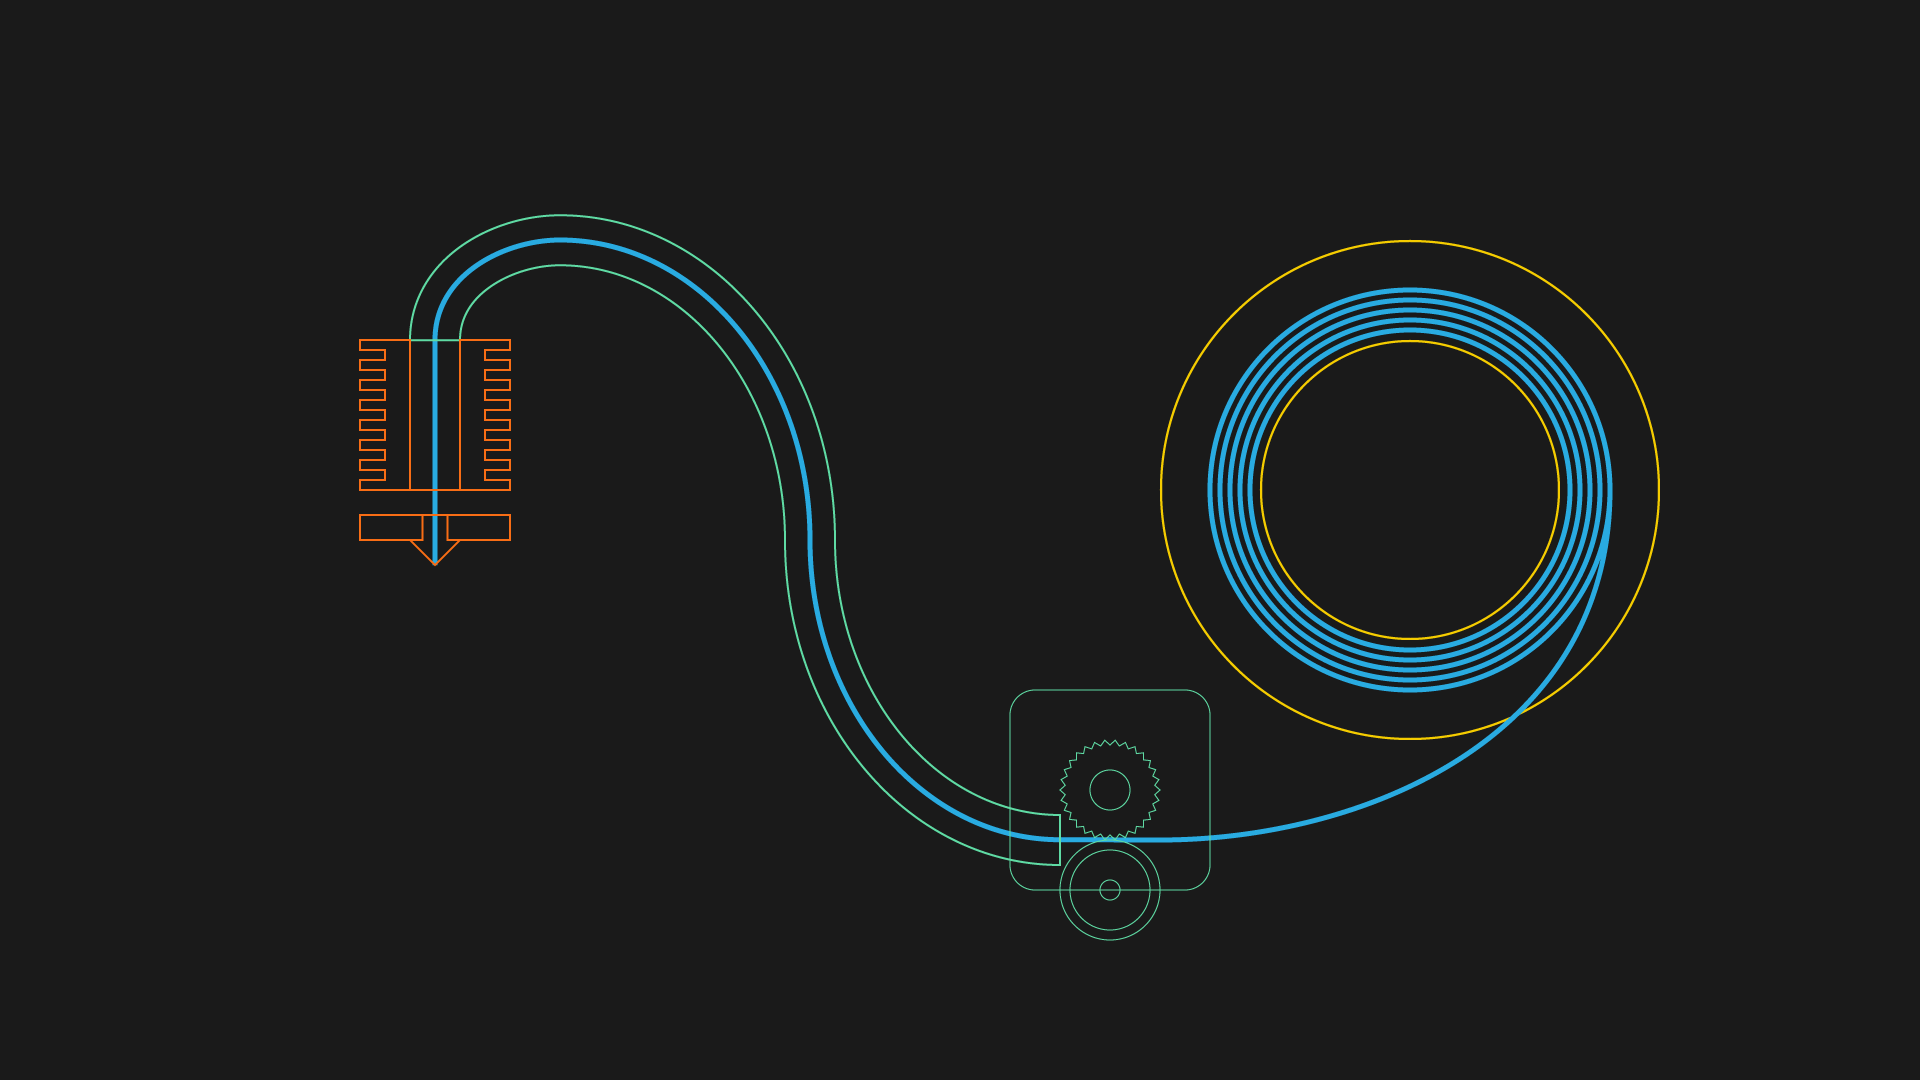
\includegraphics[width=\paperwidth]{images/extruder/bowden_drawing_colored.png}\hfil}\vfil}
}
}
\begin{frame}
  \frametitle{Wie funktioniert ein Drucker?}
\end{frame}
}
{
\usebackgroundtemplate{%
\colorbox{BackgroundJGH}{%
\vbox to \paperheight{\vfil\hbox to \paperwidth{\hfil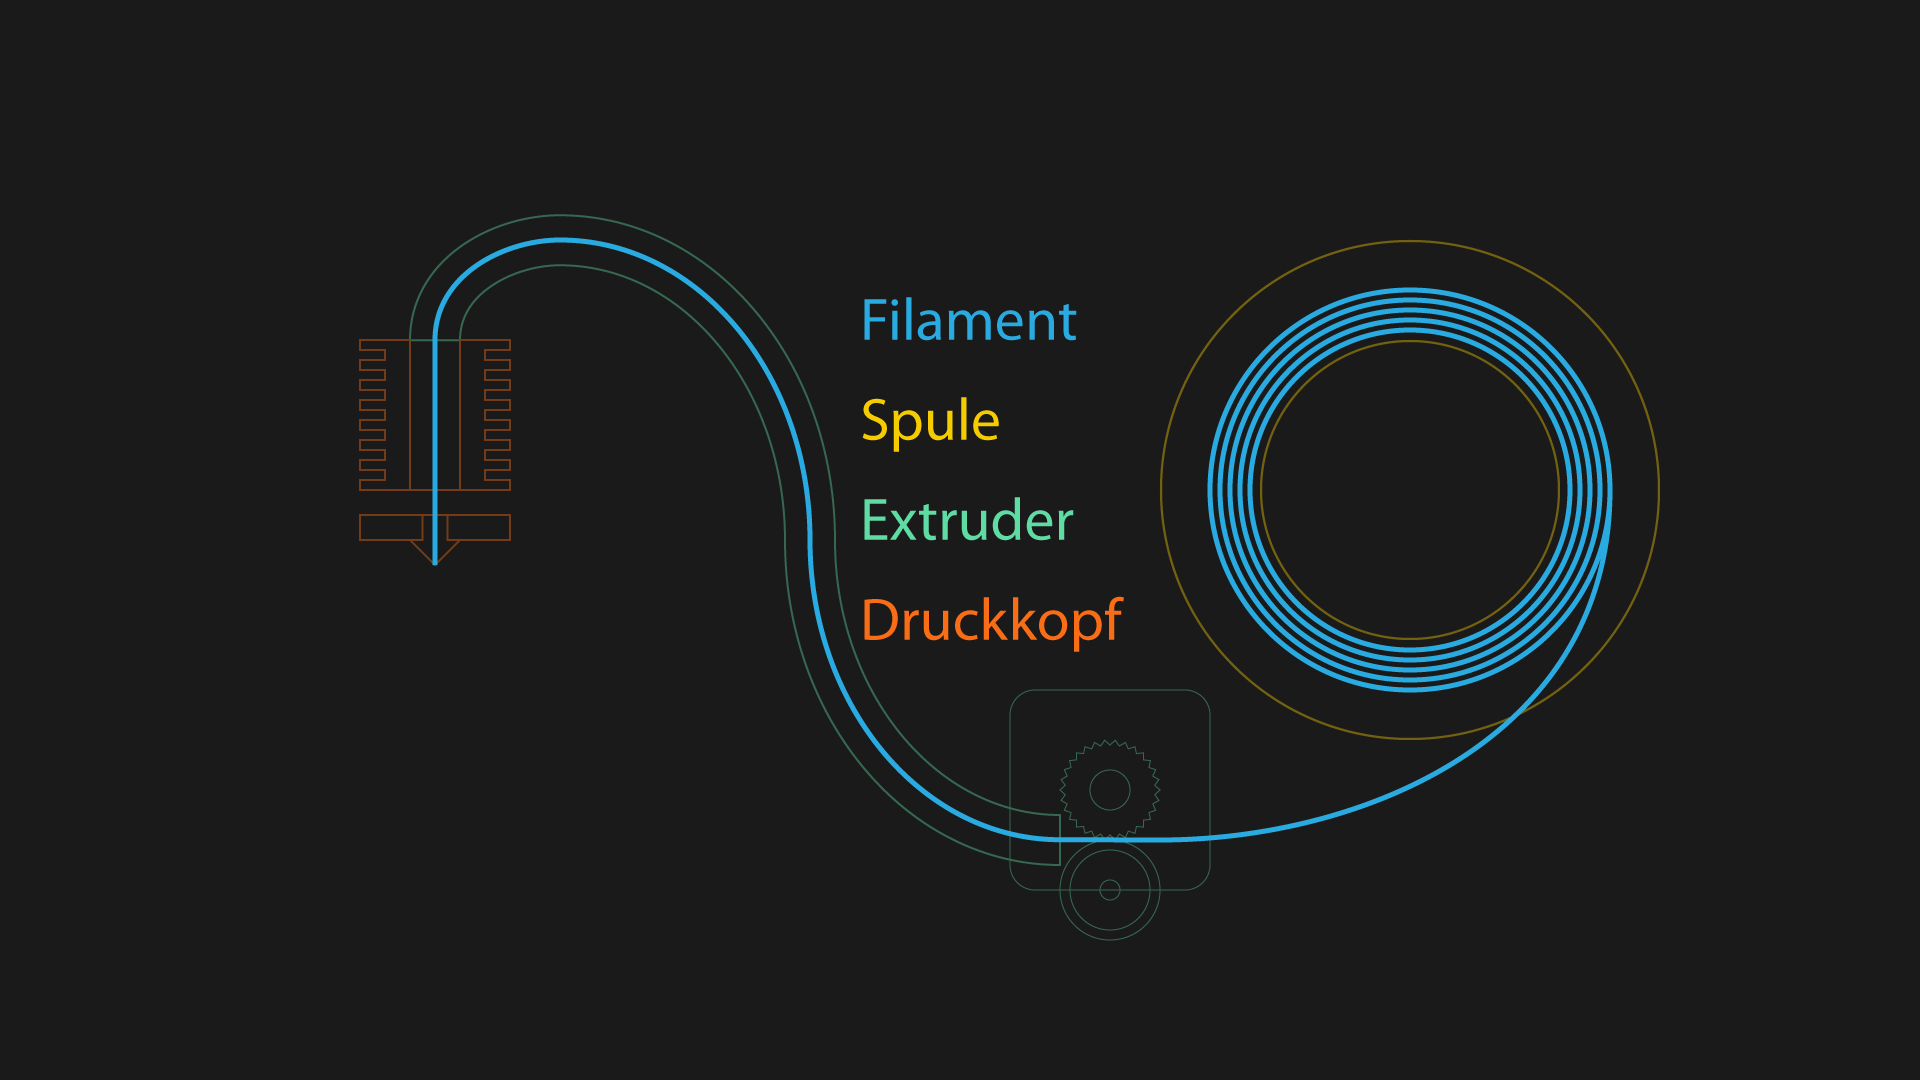
\includegraphics[width=\paperwidth]{images/extruder/filament_flow.png}\hfil}\vfil}
}
}
\subsection{Wie funktioniert das mit dem Filament?}
\begin{frame}
  \frametitle{Wie funktioniert das mit dem Filament?}
\end{frame}
}


\usebackgroundtemplate{%
\colorbox{BackgroundJGH}{%
\vbox to \paperheight{\vfil\hbox to \paperwidth{\hfil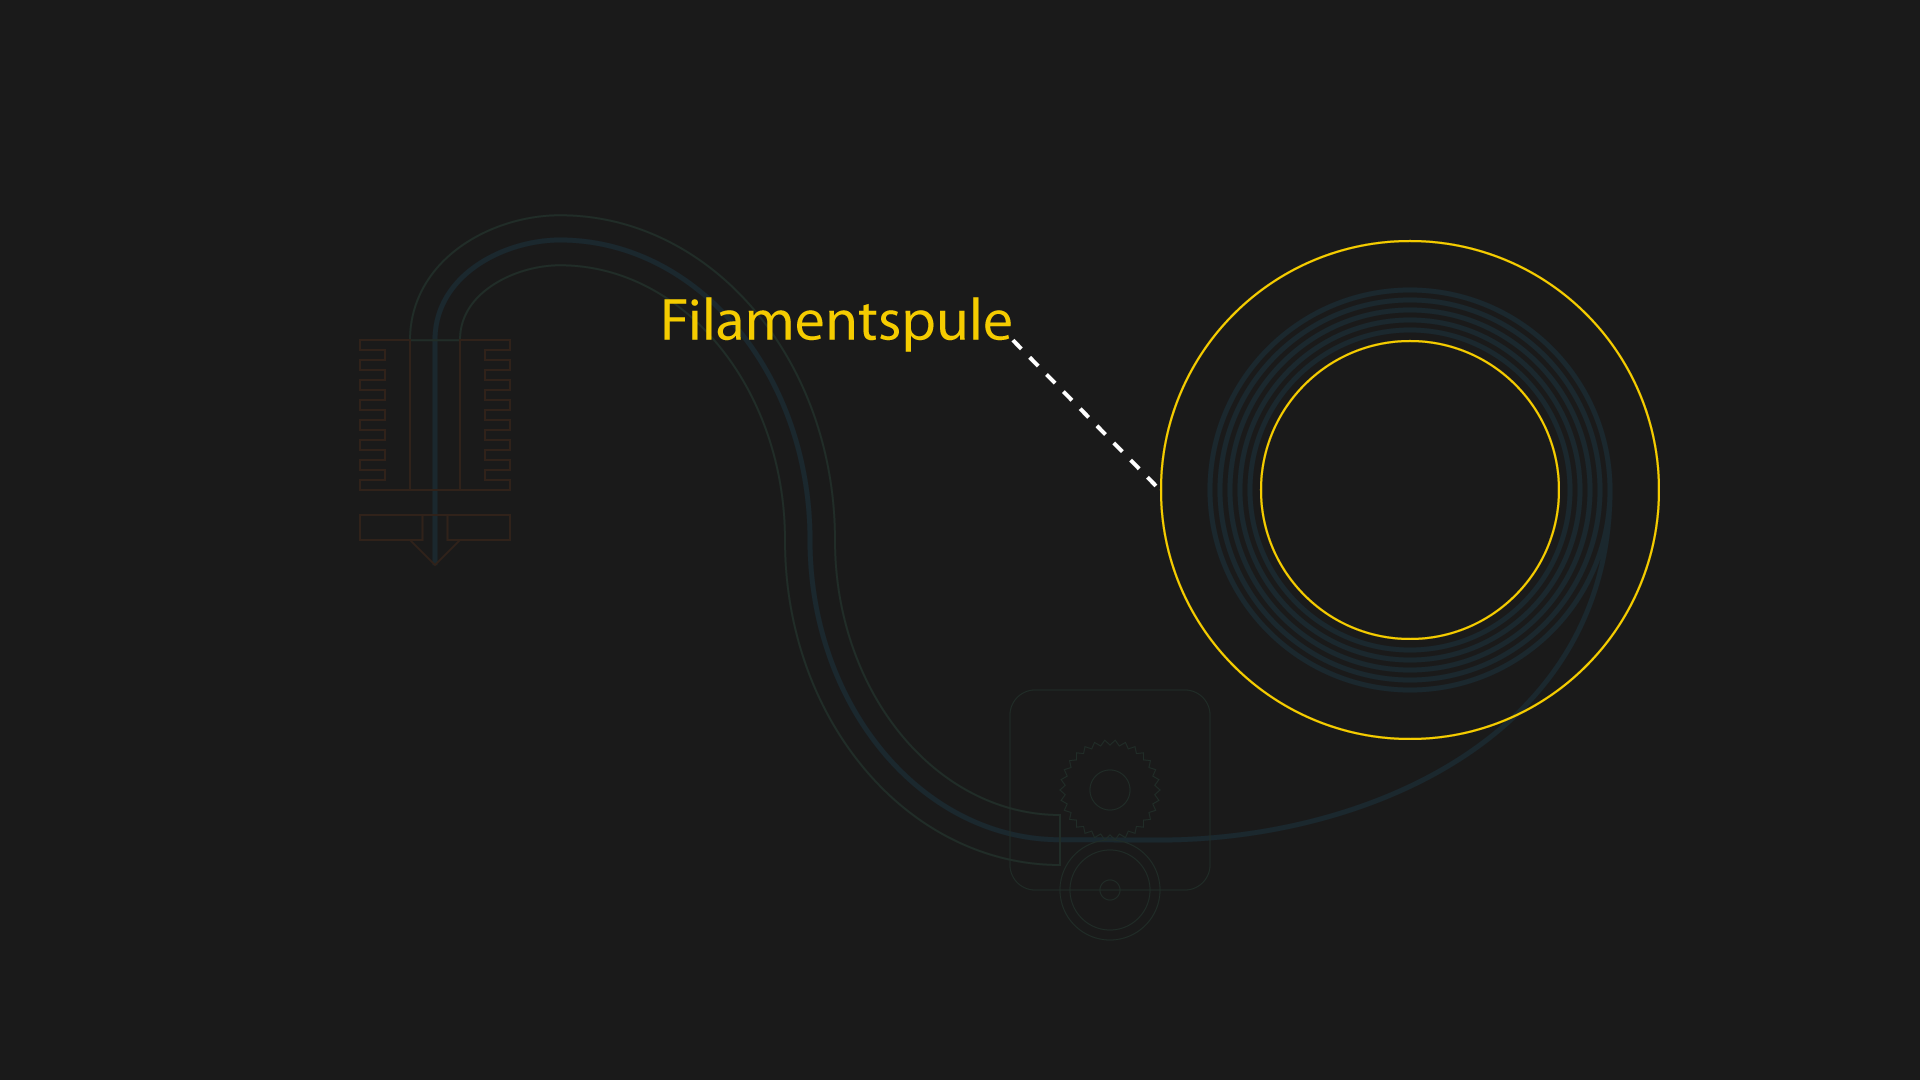
\includegraphics[width=\paperwidth]{images/extruder/filament_spool.png}\hfil}\vfil}
}
\begin{frame}
  \frametitle{Filamentspule}
\end{frame}
}
{
\usebackgroundtemplate{%
\colorbox{BackgroundJGH}{%
\vbox to \paperheight{\vfil\hbox to \paperwidth{\hfil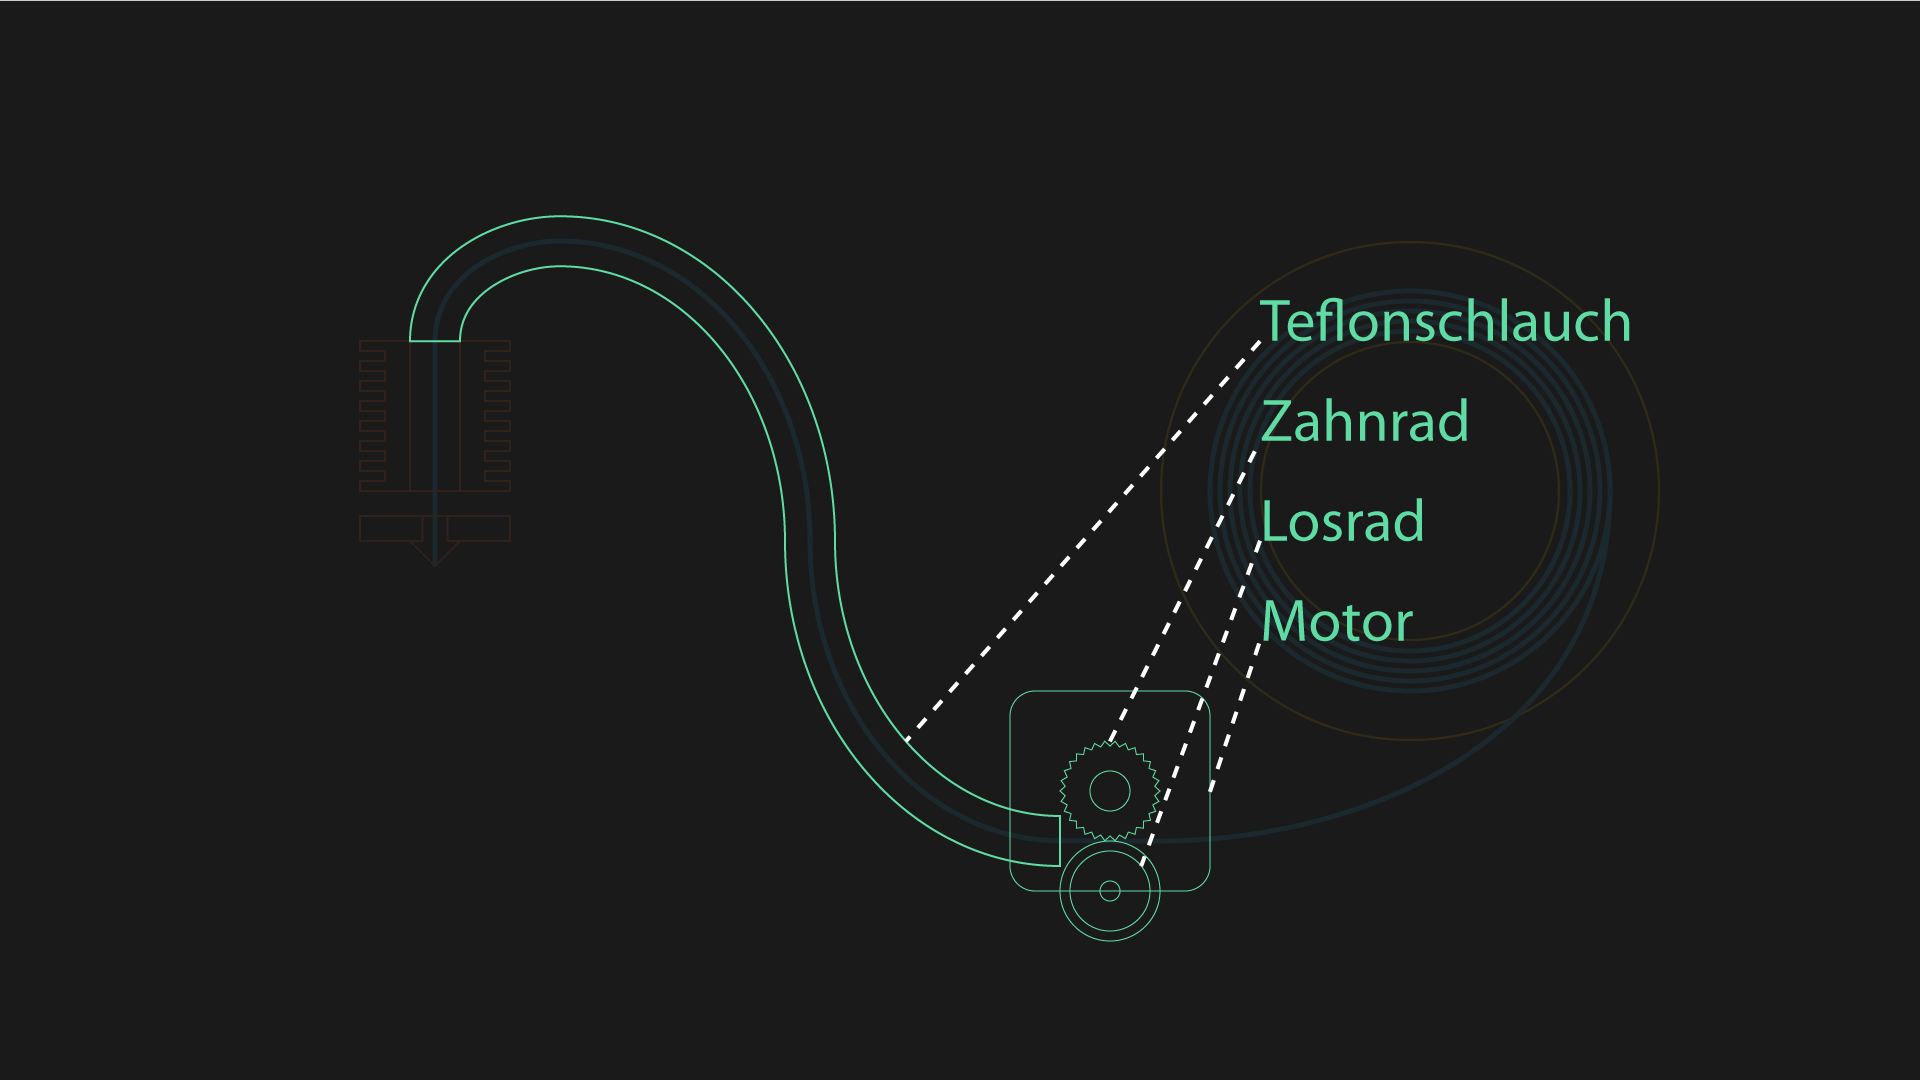
\includegraphics[width=\paperwidth]{images/extruder/bowden.png}\hfil}\vfil}
}
}
\begin{frame}
  \frametitle{Bowden Extruder}
\end{frame}
}
{
\usebackgroundtemplate{%
\colorbox{BackgroundJGH}{%
\vbox to \paperheight{\vfil\hbox to \paperwidth{\hfil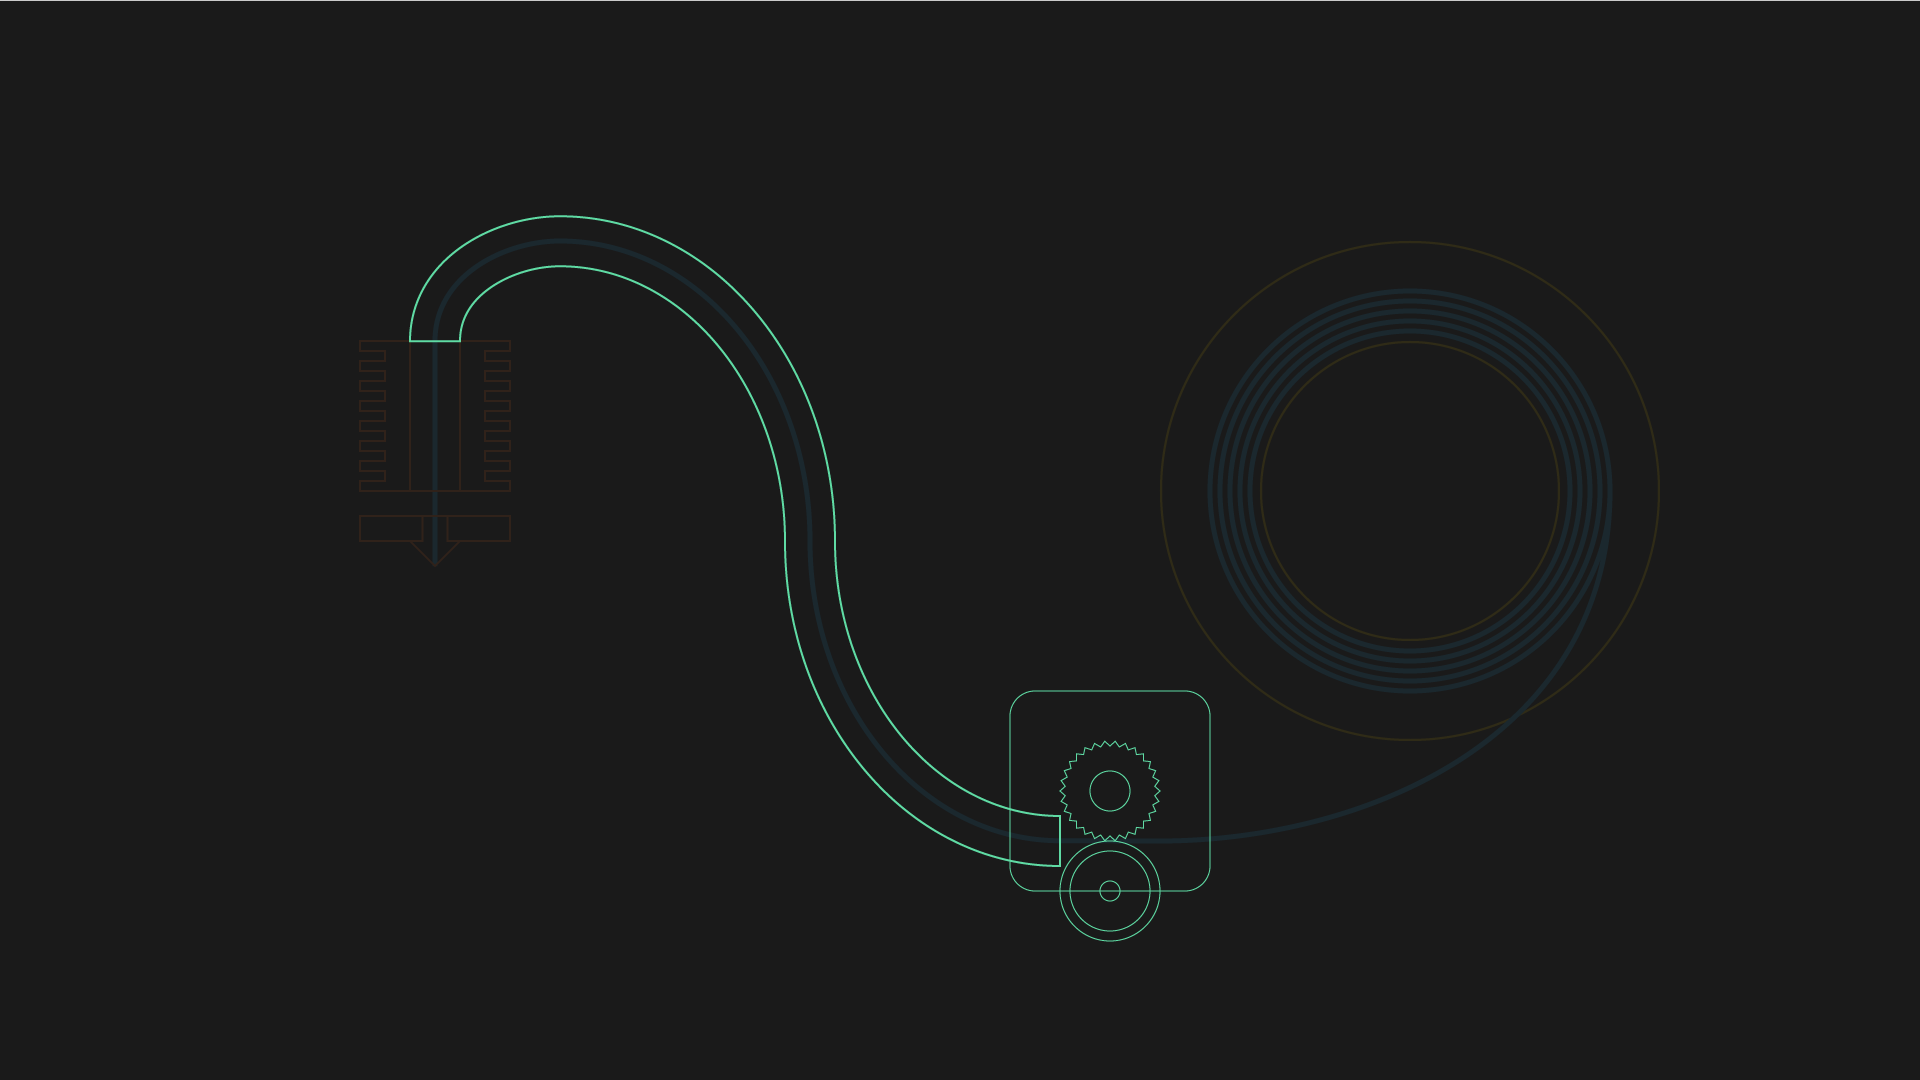
\includegraphics[width=\paperwidth]{images/extruder/bowden_no_text.png}\hfil}\vfil}
}
}
\begin{frame}
  \frametitle{Bowden Extruder}
  \pause
  \begin{itemize}
    \item Leicht zu tauschen \pause
    \item Weniger Masse am Druckkopf
    \begin{itemize}
      \item Schnellere Bewegungen
      \item Schnellere Druckgeschwindigkeit
      \item Höhere Genauigkeit \pause
    \end{itemize}
    \item Langer Bowdentube
    \begin{itemize}
      \item Reibung
      \item Dehnung/Stauchung des Filaments
    \end{itemize}
  \end{itemize}
\end{frame}
}
{
\usebackgroundtemplate{%
\colorbox{BackgroundJGH}{%
\vbox to \paperheight{\vfil\hbox to \paperwidth{\hfil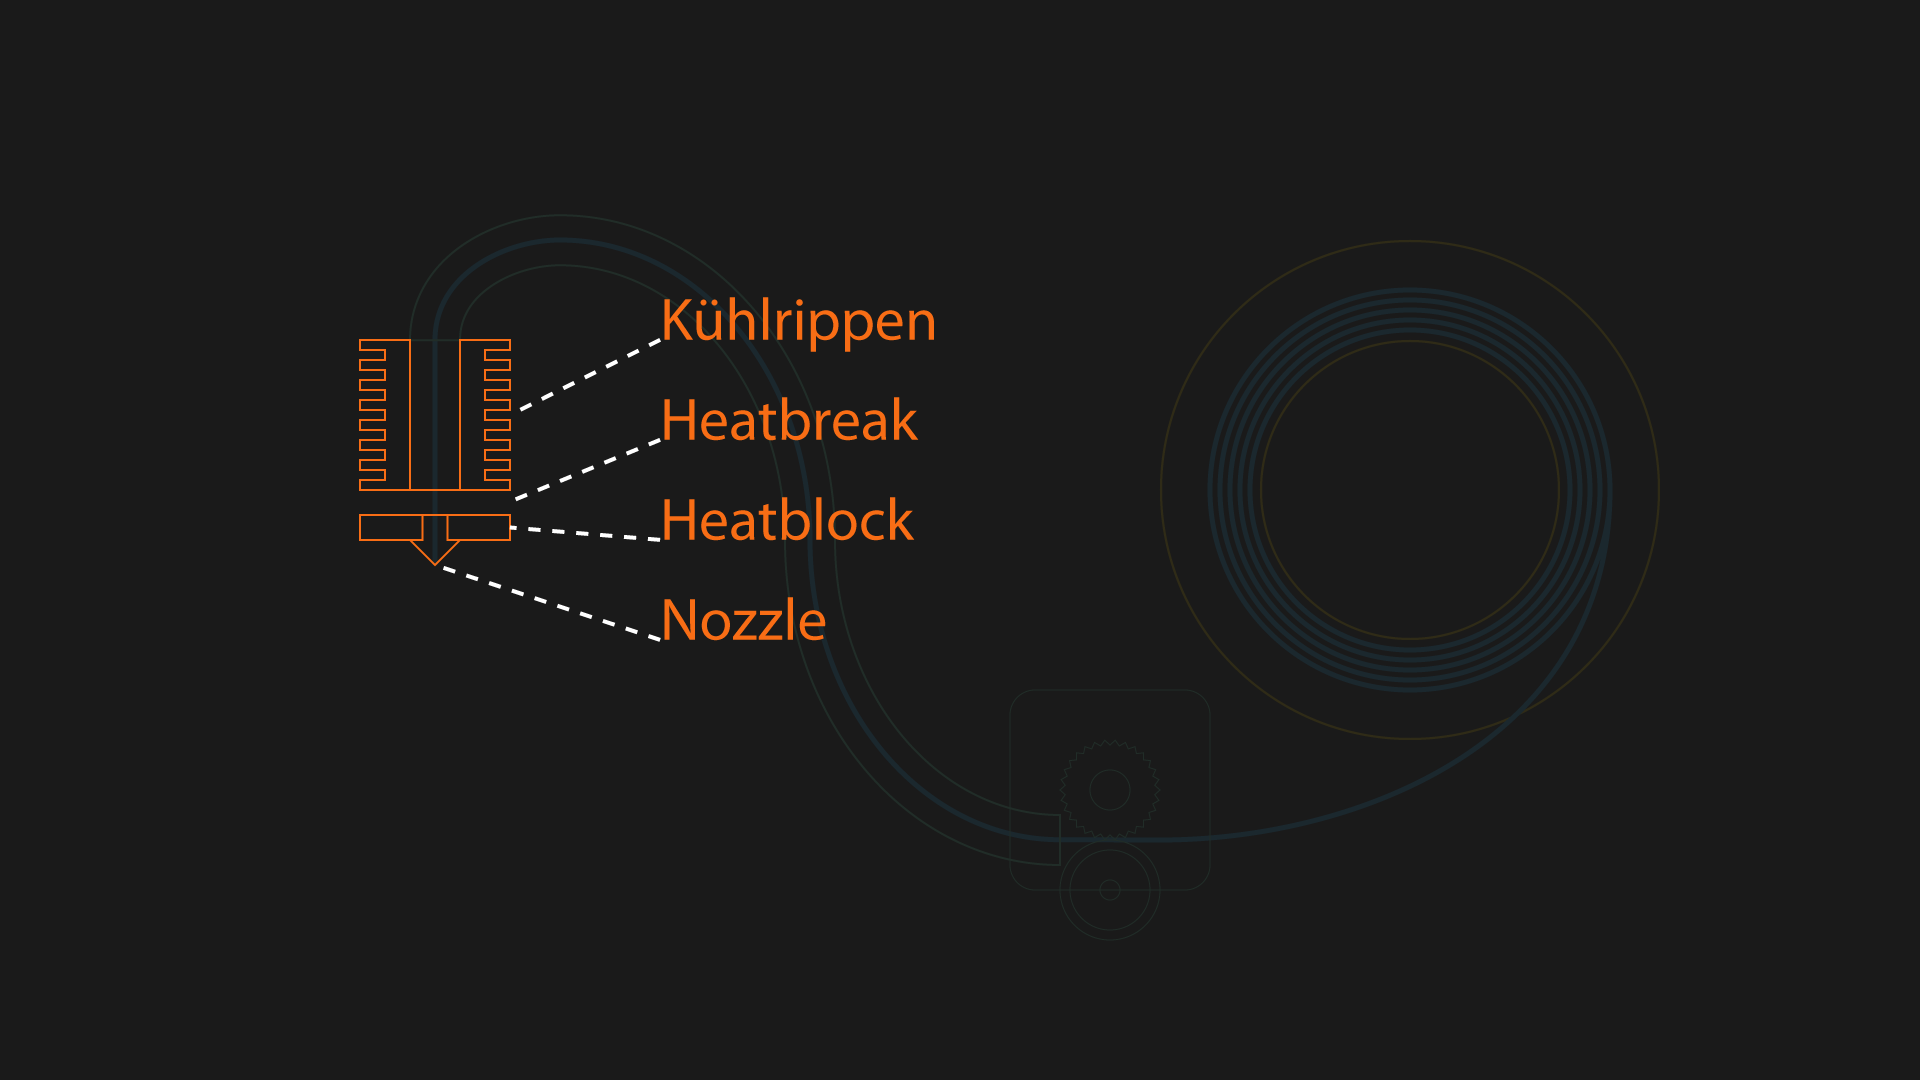
\includegraphics[width=\paperwidth]{images/extruder/print_head.png}\hfil}\vfil}
}
}
\begin{frame}
  \frametitle{Druckkopf}
\end{frame}
}
{
\usebackgroundtemplate{%
\colorbox{BackgroundJGH}{%
\vbox to \paperheight{\vfil\hbox to \paperwidth{\hfil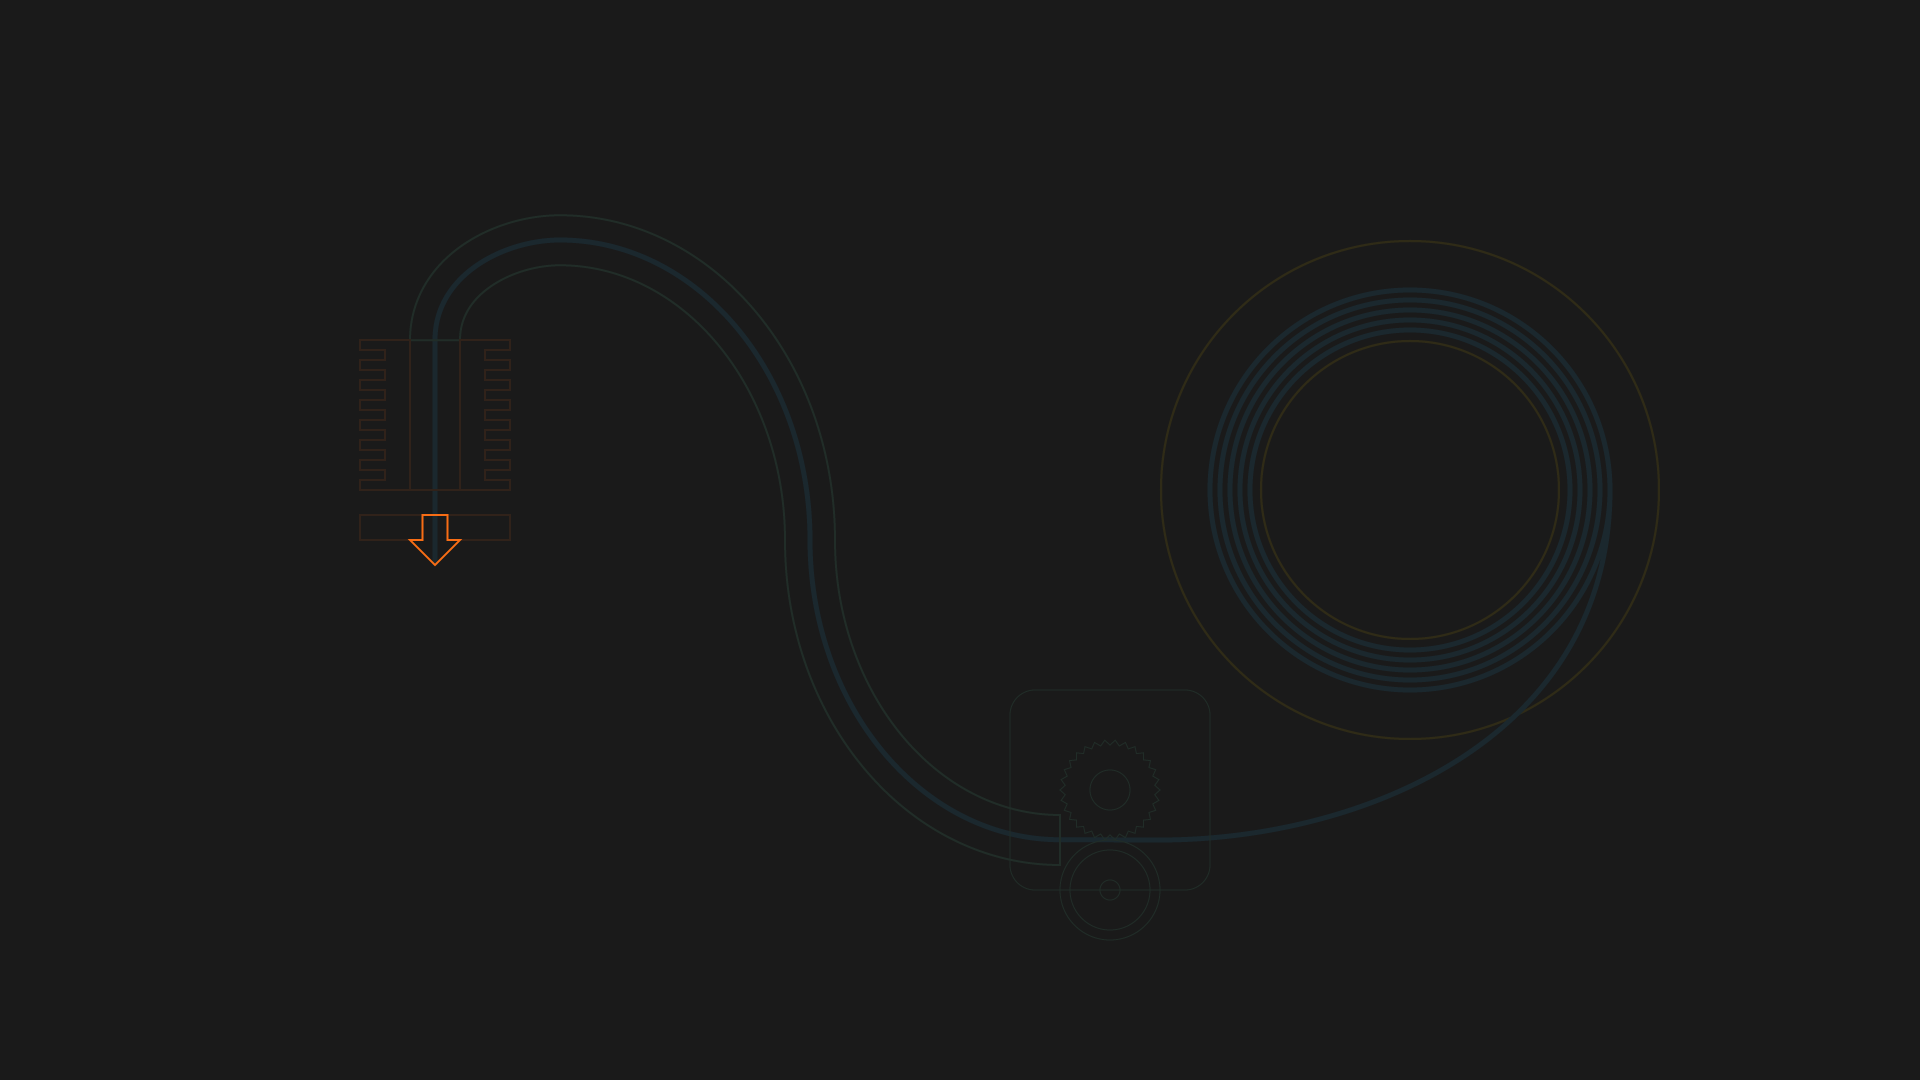
\includegraphics[width=\paperwidth]{images/extruder/nozzle.png}\hfil}\vfil}
}
}
\begin{frame}
  \frametitle{Nozzle}
  \pause
  \begin{itemize}
    \item Wird nach der Größe der Öffnung benannt \pause
    \item Meist 0.4mm Durchmesser \pause
    \item Gibt Schichtdicke und Wandbreite vor \pause
    \begin{itemize}
      \item 0.4mm ermöglicht 0.1-0.3mm Schichtdicke
      \item Wandstärke immer ein Vielfaches des Nozzledurchmessers
      \item Höhen immer ein Vielfaches der Schichtdicke
    \end{itemize}
  \end{itemize}
\end{frame}
}

\subsection{Wie wird der Druckkopf bewegt?}
{
\usebackgroundtemplate{%
\colorbox{BackgroundJGH}{%
\vbox to \paperheight{\vfil\hbox to \paperwidth{\hfil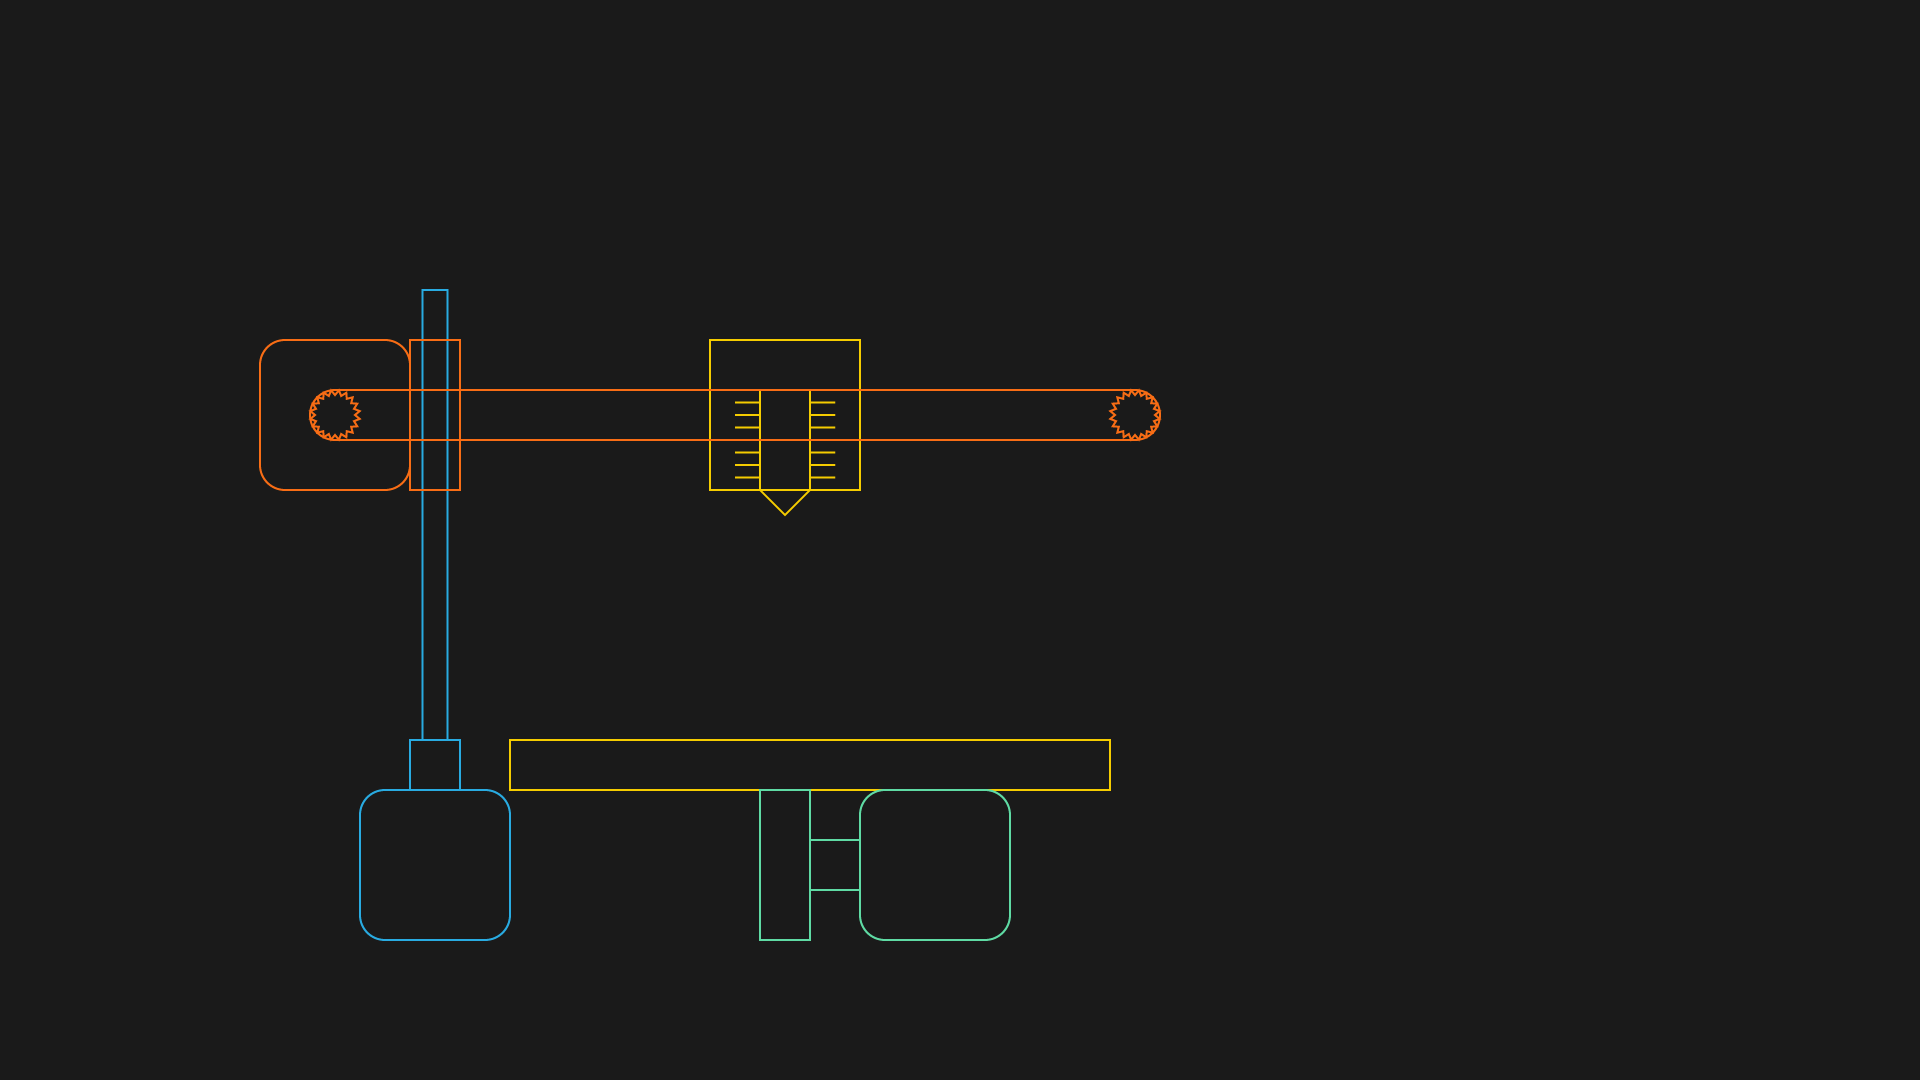
\includegraphics[width=\paperwidth]{images/mechanik/complete.png}\hfil}\vfil}
}
}
\begin{frame}
  \frametitle{Wie wird der Druckkopf bewegt?}
\end{frame}
}

{
\usebackgroundtemplate{%
\colorbox{BackgroundJGH}{%
\vbox to \paperheight{\vfil\hbox to \paperwidth{\hfil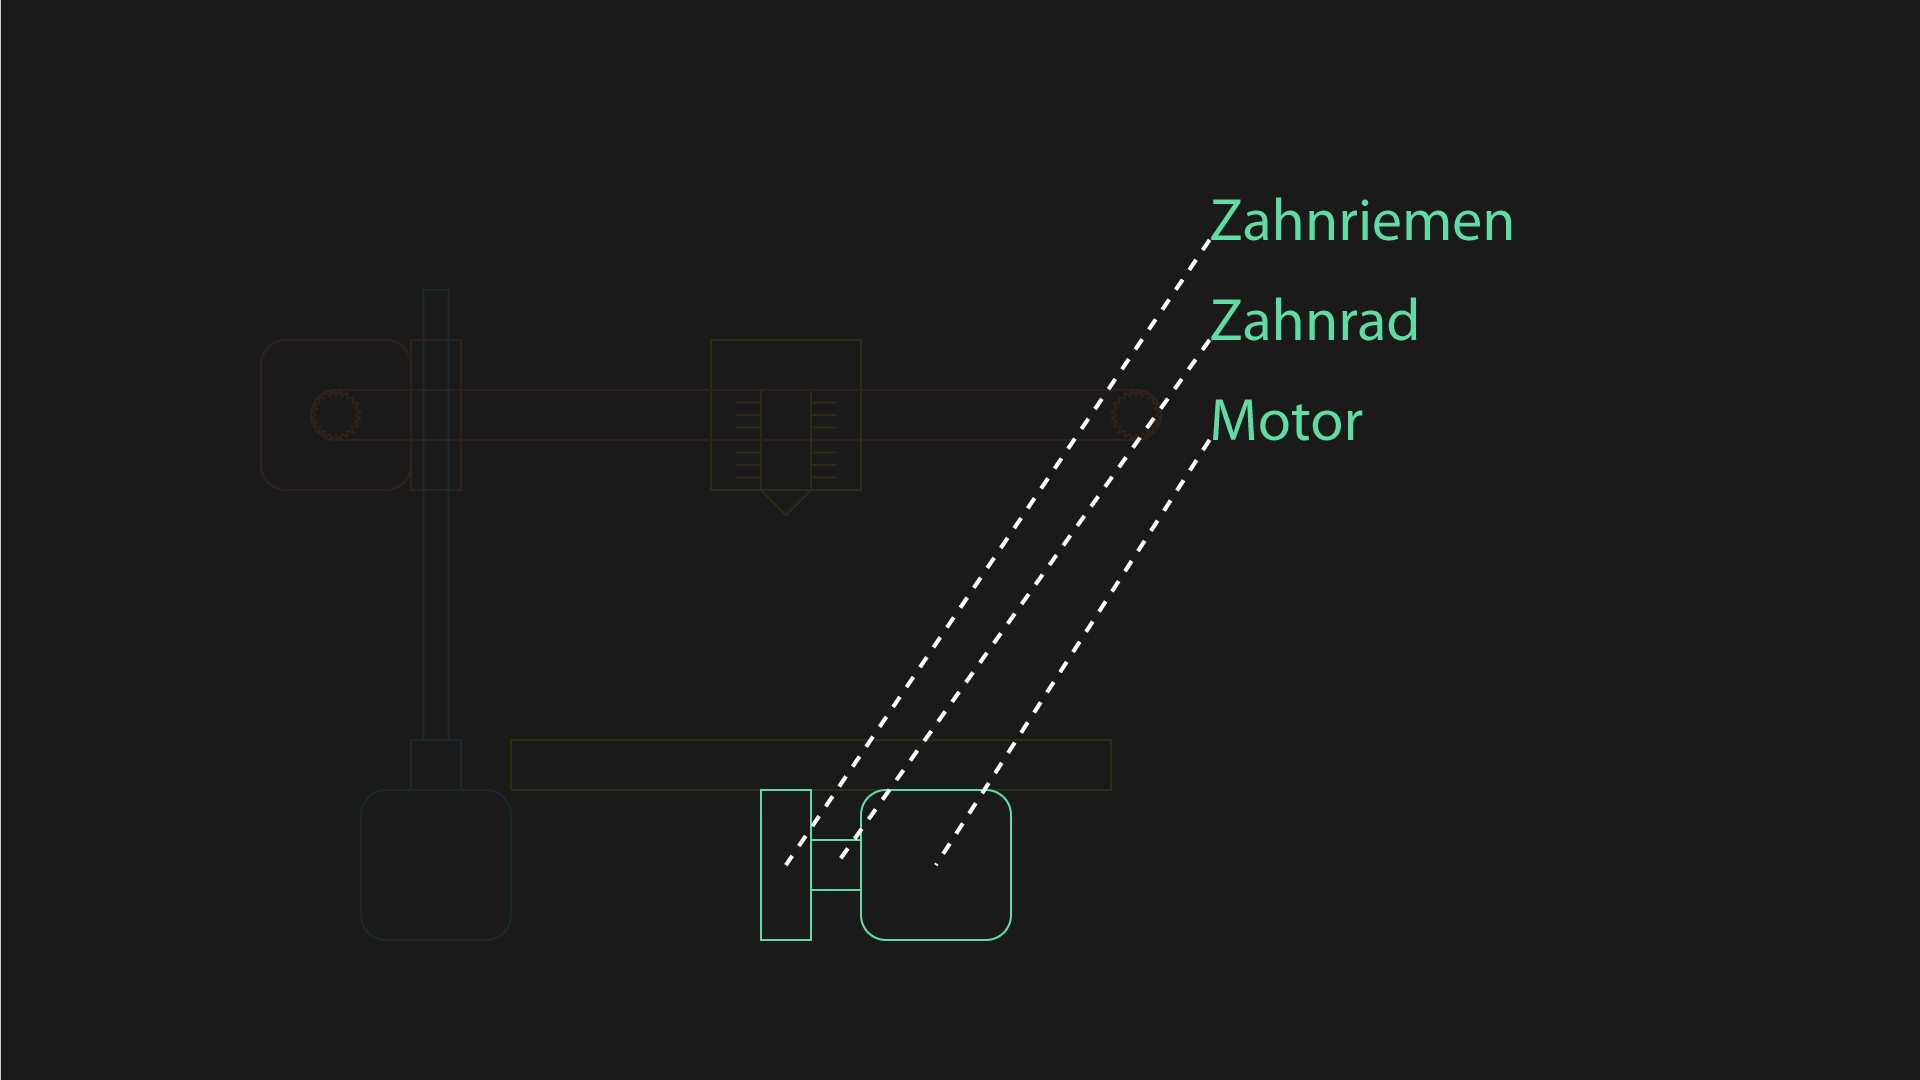
\includegraphics[width=\paperwidth]{images/mechanik/y-axis.png}\hfil}\vfil}
}
}
\begin{frame}
  \frametitle{Y-Achse}
\end{frame}
}

{
\usebackgroundtemplate{%
\colorbox{BackgroundJGH}{%
\vbox to \paperheight{\vfil\hbox to \paperwidth{\hfil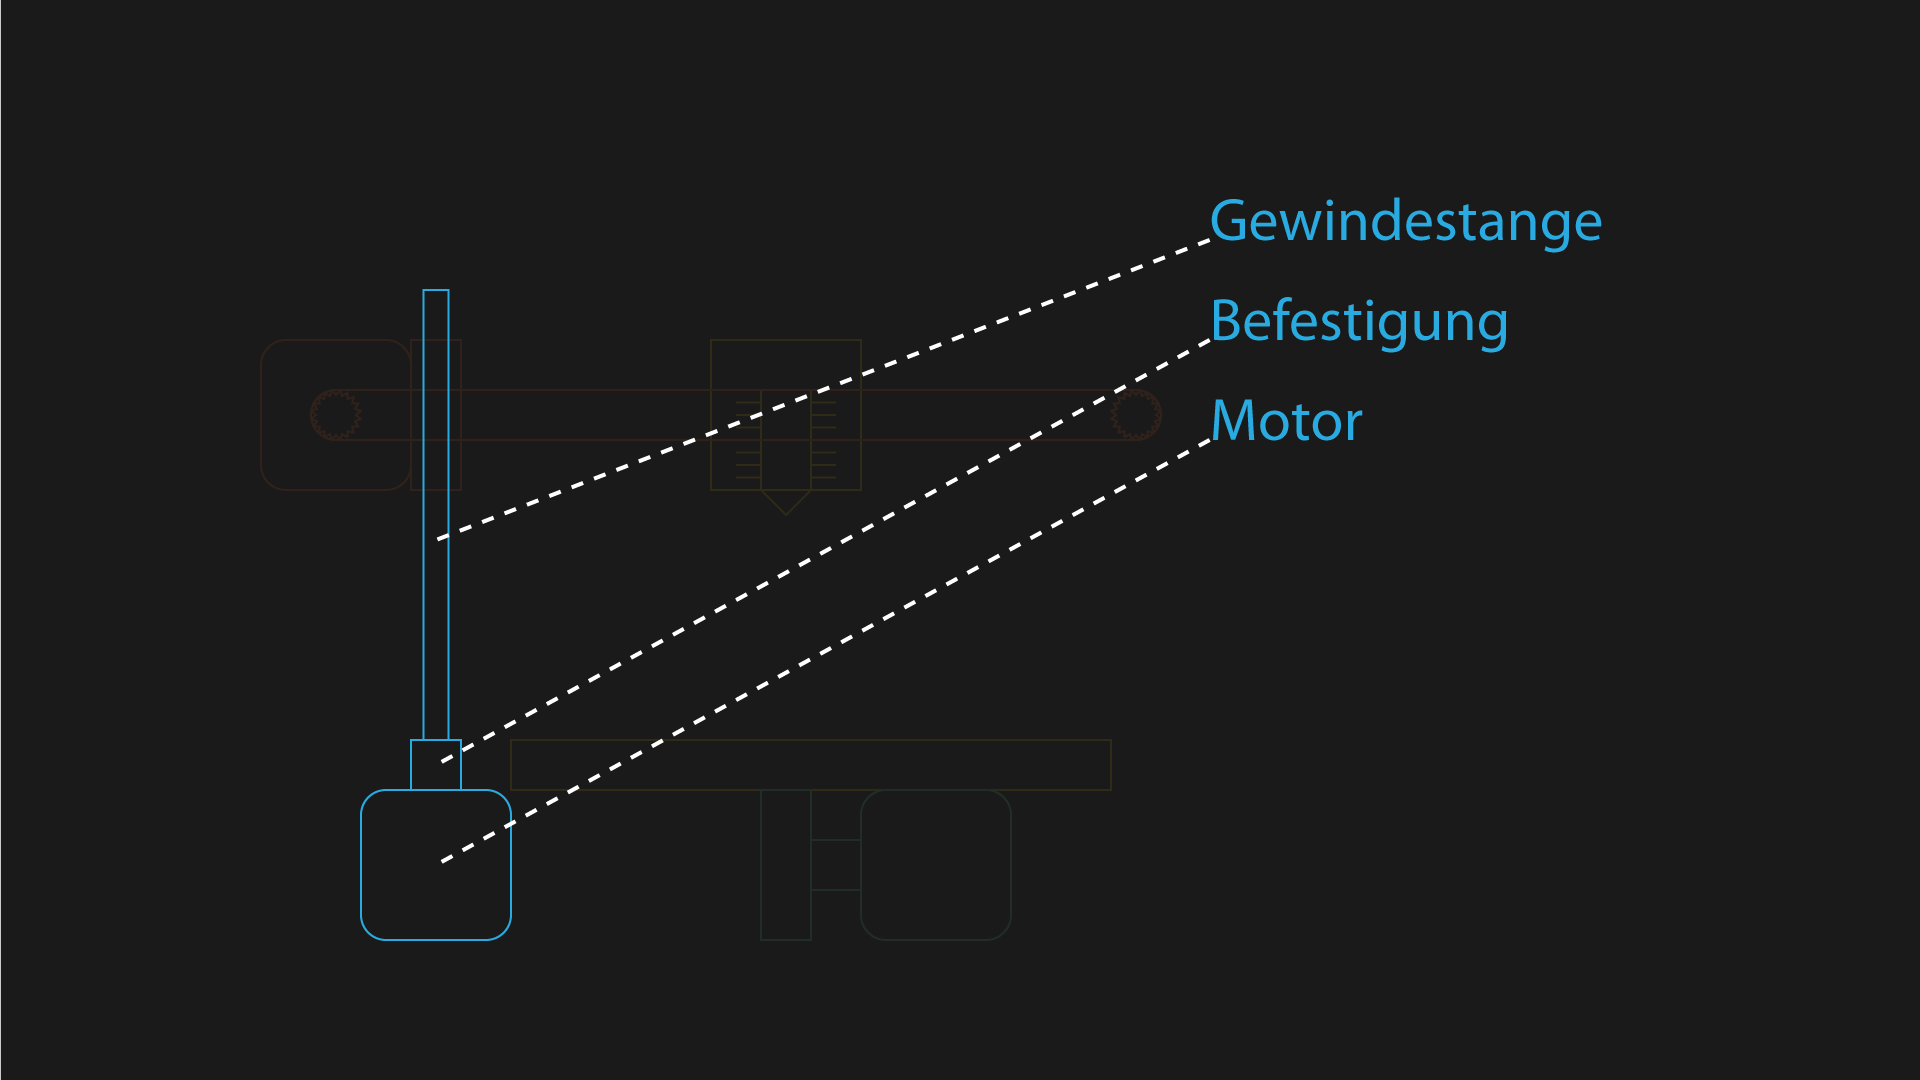
\includegraphics[width=\paperwidth]{images/mechanik/z-axis.png}\hfil}\vfil}
}
}
\begin{frame}
  \frametitle{Z-Achse}
\end{frame}
}

{
\usebackgroundtemplate{%
\colorbox{BackgroundJGH}{%
\vbox to \paperheight{\vfil\hbox to \paperwidth{\hfil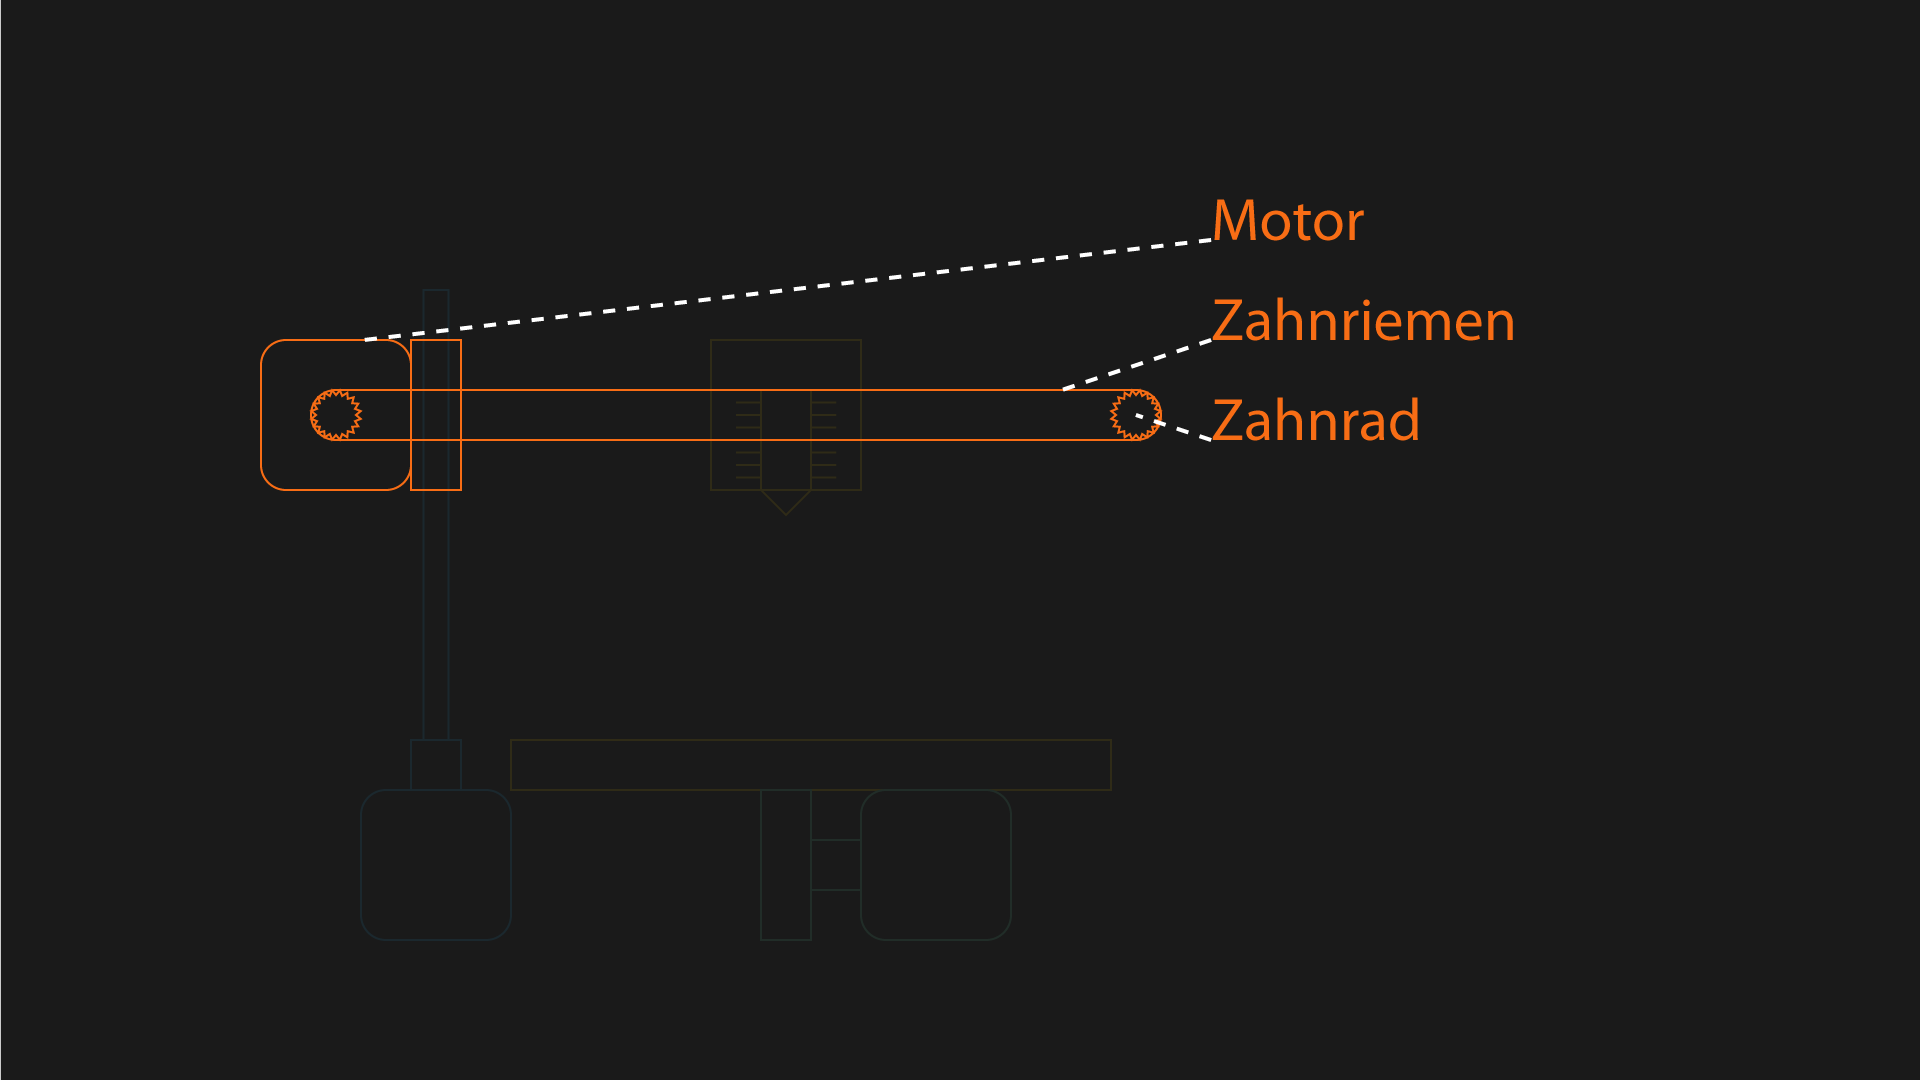
\includegraphics[width=\paperwidth]{images/mechanik/x-axis.png}\hfil}\vfil}
}
}
\begin{frame}
  \frametitle{X-Achse}
\end{frame}
}

{
\usebackgroundtemplate{%
\colorbox{BackgroundJGH}{%
\vbox to \paperheight{\vfil\hbox to \paperwidth{\hfil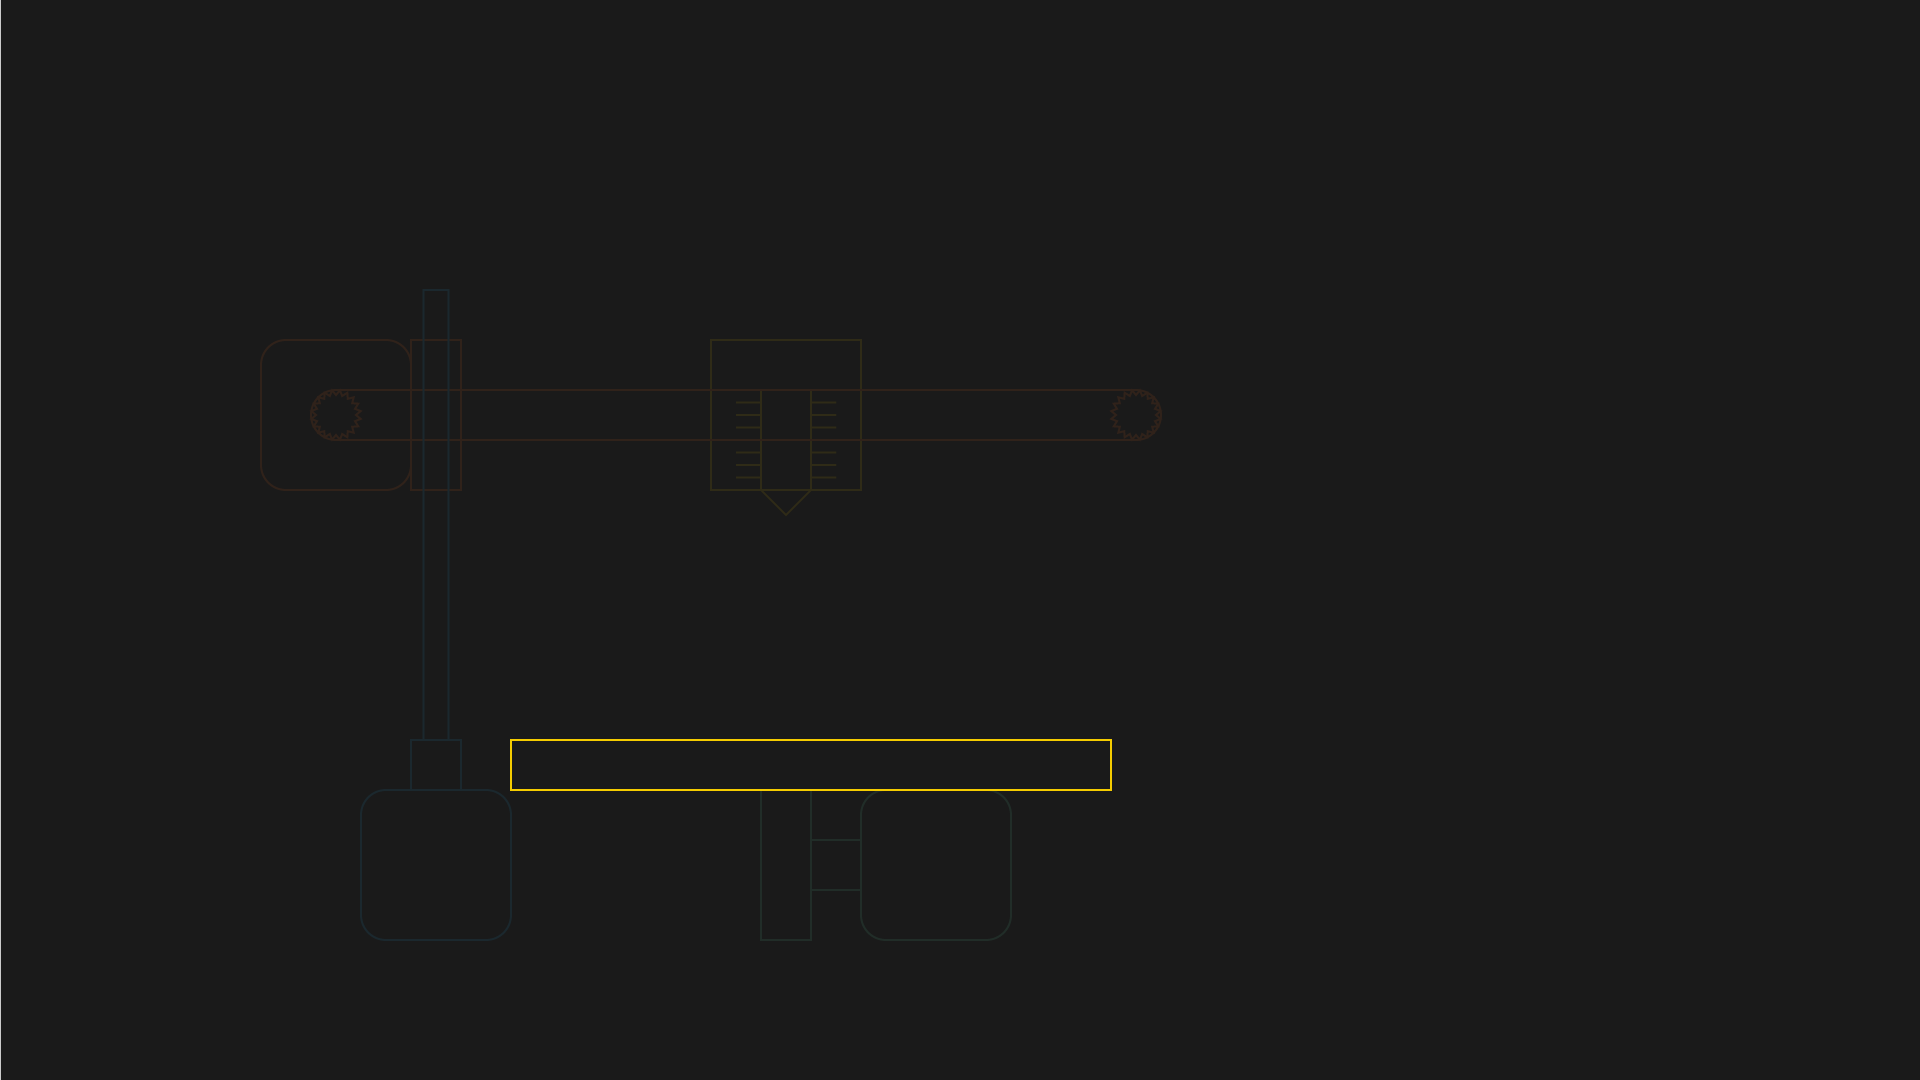
\includegraphics[width=\paperwidth]{images/mechanik/print_bed.png}\hfil}\vfil}
}
}
\begin{frame}
  \frametitle{Druckbett}
  \pause
  \begin{itemize}
    \item Beheizt \pause
    \item Unbeheizt
  \end{itemize}
\end{frame}

\begin{frame}
  \frametitle{Druckbett}
  \begin{itemize}
    \item Glas \pause
    \begin{itemize}
      \item Viele Materialien nur Beheizt
      \item Glastemperatur \pause
    \end{itemize}
    \item Kunststoffe \pause
    \begin{itemize}
      \item Oft mit strukturierter Oberfläche \pause
    \end{itemize}
    \item Bluetape \pause
    \begin{itemize}
      \item Oft zum Verbessern der Haftung verwendet
    \end{itemize}
  \end{itemize}
\end{frame}
}
